La síntesis final clasifica las regiones Mapper según el tipo de evidencia que las sostiene. Esta clasificación no se aplica a planetas individuales ni busca construir una taxonomía final de exoplanetas. En cambio, clasifica nodos y componentes del grafo como regiones de evidencia: algunas tienen una interpretación física u orbital más limpia, otras están dominadas por variables observacionales, otras mezclan señal astrofísica y sesgo de descubrimiento, y otras no tienen suficiente soporte para ser interpretadas con confianza.

La pregunta central de esta sección es:

\begin{quote}
Después de construir Mapper, auditar imputación y auditar sesgo observacional, ¿qué tipo de regiones encontramos realmente?
\end{quote}

Para responderla, cada región se evaluó combinando cuatro fuentes de evidencia: coherencia física, orbital o térmica; enriquecimiento por \texttt{discoverymethod}; riesgo de imputación; y tamaño o confiabilidad de la región. Esta lectura permite evitar una interpretación demasiado directa de los grafos. Una región puede verse estructurada en Mapper, pero si está dominada por un método de descubrimiento, por una instalación específica o por valores altamente imputados, su interpretación astrofísica debe moderarse.

Las categorías finales son:

\begin{itemize}
    \item \texttt{physical}: regiones con coherencia física u orbital, baja imputación y baja evidencia de sesgo observacional.
    \item \texttt{observational}: regiones dominadas por método de descubrimiento, facilidad, época o enriquecimiento observacional significativo.
    \item \texttt{mixed}: regiones con alguna coherencia física u orbital, pero también con señal observacional relevante.
    \item \texttt{weak}: regiones con alta imputación, tamaño pequeño, evidencia conflictiva o soporte insuficiente para una interpretación fuerte.
\end{itemize}

Estas etiquetas no son clases planetarias. Son categorías de evidencia. Por ejemplo, una región \texttt{physical} no significa que se descubrió una nueva familia de planetas, sino que esa región tiene evidencia relativamente limpia para inspección astrofísica posterior. Del mismo modo, una región \texttt{mixed} no significa que no tenga señal física; significa que esa señal aparece entrelazada con sesgo observacional o incertidumbre metodológica.

\begin{table}[H]
\centering
\small
\begin{tabular}{lrrp{0.43\textwidth}}
\toprule
\textbf{Categoría} & \textbf{Nodos} & \textbf{Componentes} & \textbf{Lectura} \\
\midrule
\texttt{physical} & 10 & 0 & Regiones con evidencia física u orbital relativamente limpia. \\
\texttt{observational} & 1 & 4 & Regiones dominadas por señal observacional. \\
\texttt{mixed} & 240 & 36 & Regiones con señal física/orbital mezclada con sesgo observacional. \\
\texttt{weak} & 245 & 70 & Regiones con evidencia insuficiente, alta imputación o interpretación débil. \\
\bottomrule
\end{tabular}
\caption{Conteo final de regiones Mapper por tipo de evidencia.}
\label{tab:final_region_counts}
\end{table}

La Tabla~\ref{tab:final_region_counts} muestra que la mayor parte de la estructura no cae en una categoría puramente física. Solo 10 nodos fueron clasificados como \texttt{physical}, mientras que 240 nodos quedaron como \texttt{mixed} y 245 como \texttt{weak}. A nivel de componentes, predominan nuevamente las regiones \texttt{mixed} y \texttt{weak}. Esta distribución es uno de los resultados más importantes del proyecto: la topología observada no debe interpretarse como señal astrofísica limpia en bloque. Más bien, debe leerse como una mezcla de estructura física u orbital, sesgo observacional, imputación y sensibilidad metodológica.

\begin{figure}[H]
\centering
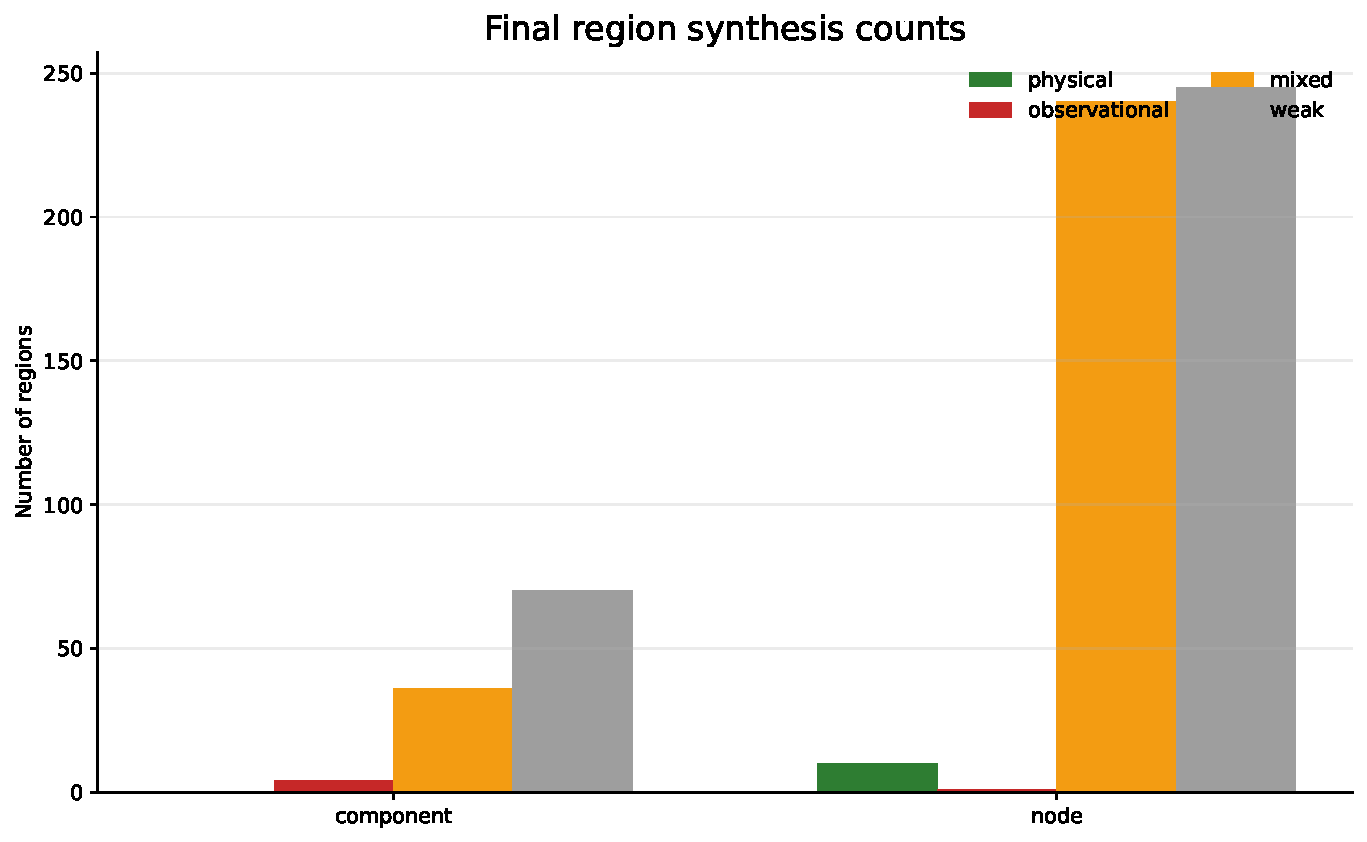
\includegraphics[width=0.78\linewidth]{figures/region_class_counts.pdf}
\caption{Conteos finales de regiones Mapper por categoría de evidencia. La figura resume la diferencia entre regiones \texttt{physical}, \texttt{observational}, \texttt{mixed} y \texttt{weak} a nivel de nodos y componentes.}
\label{fig:region_class_counts}
\end{figure}

La Figura~\ref{fig:region_class_counts} deja claro que el resultado dominante no es una colección de regiones físicas limpias, sino una abundancia de regiones mixtas y débiles. Esto no debilita el proyecto; al contrario, muestra que la auditoría era necesaria. Sin esta clasificación, sería fácil sobreinterpretar regiones estructuradas como familias planetarias, cuando en realidad muchas de ellas combinan señal física con sesgo de detección o incertidumbre de imputación.

\subsection*{Visualización de las regiones por tipo de evidencia}

La clasificación final también puede observarse directamente sobre los grafos seleccionados. La Figura~\ref{fig:main_graphs_by_evidence_class} muestra los seis grafos principales coloreados por categoría final de evidencia. Esta visualización permite comparar en una sola imagen qué tipo de regiones dominan en cada espacio de variables.

\begin{figure}[H]
\centering
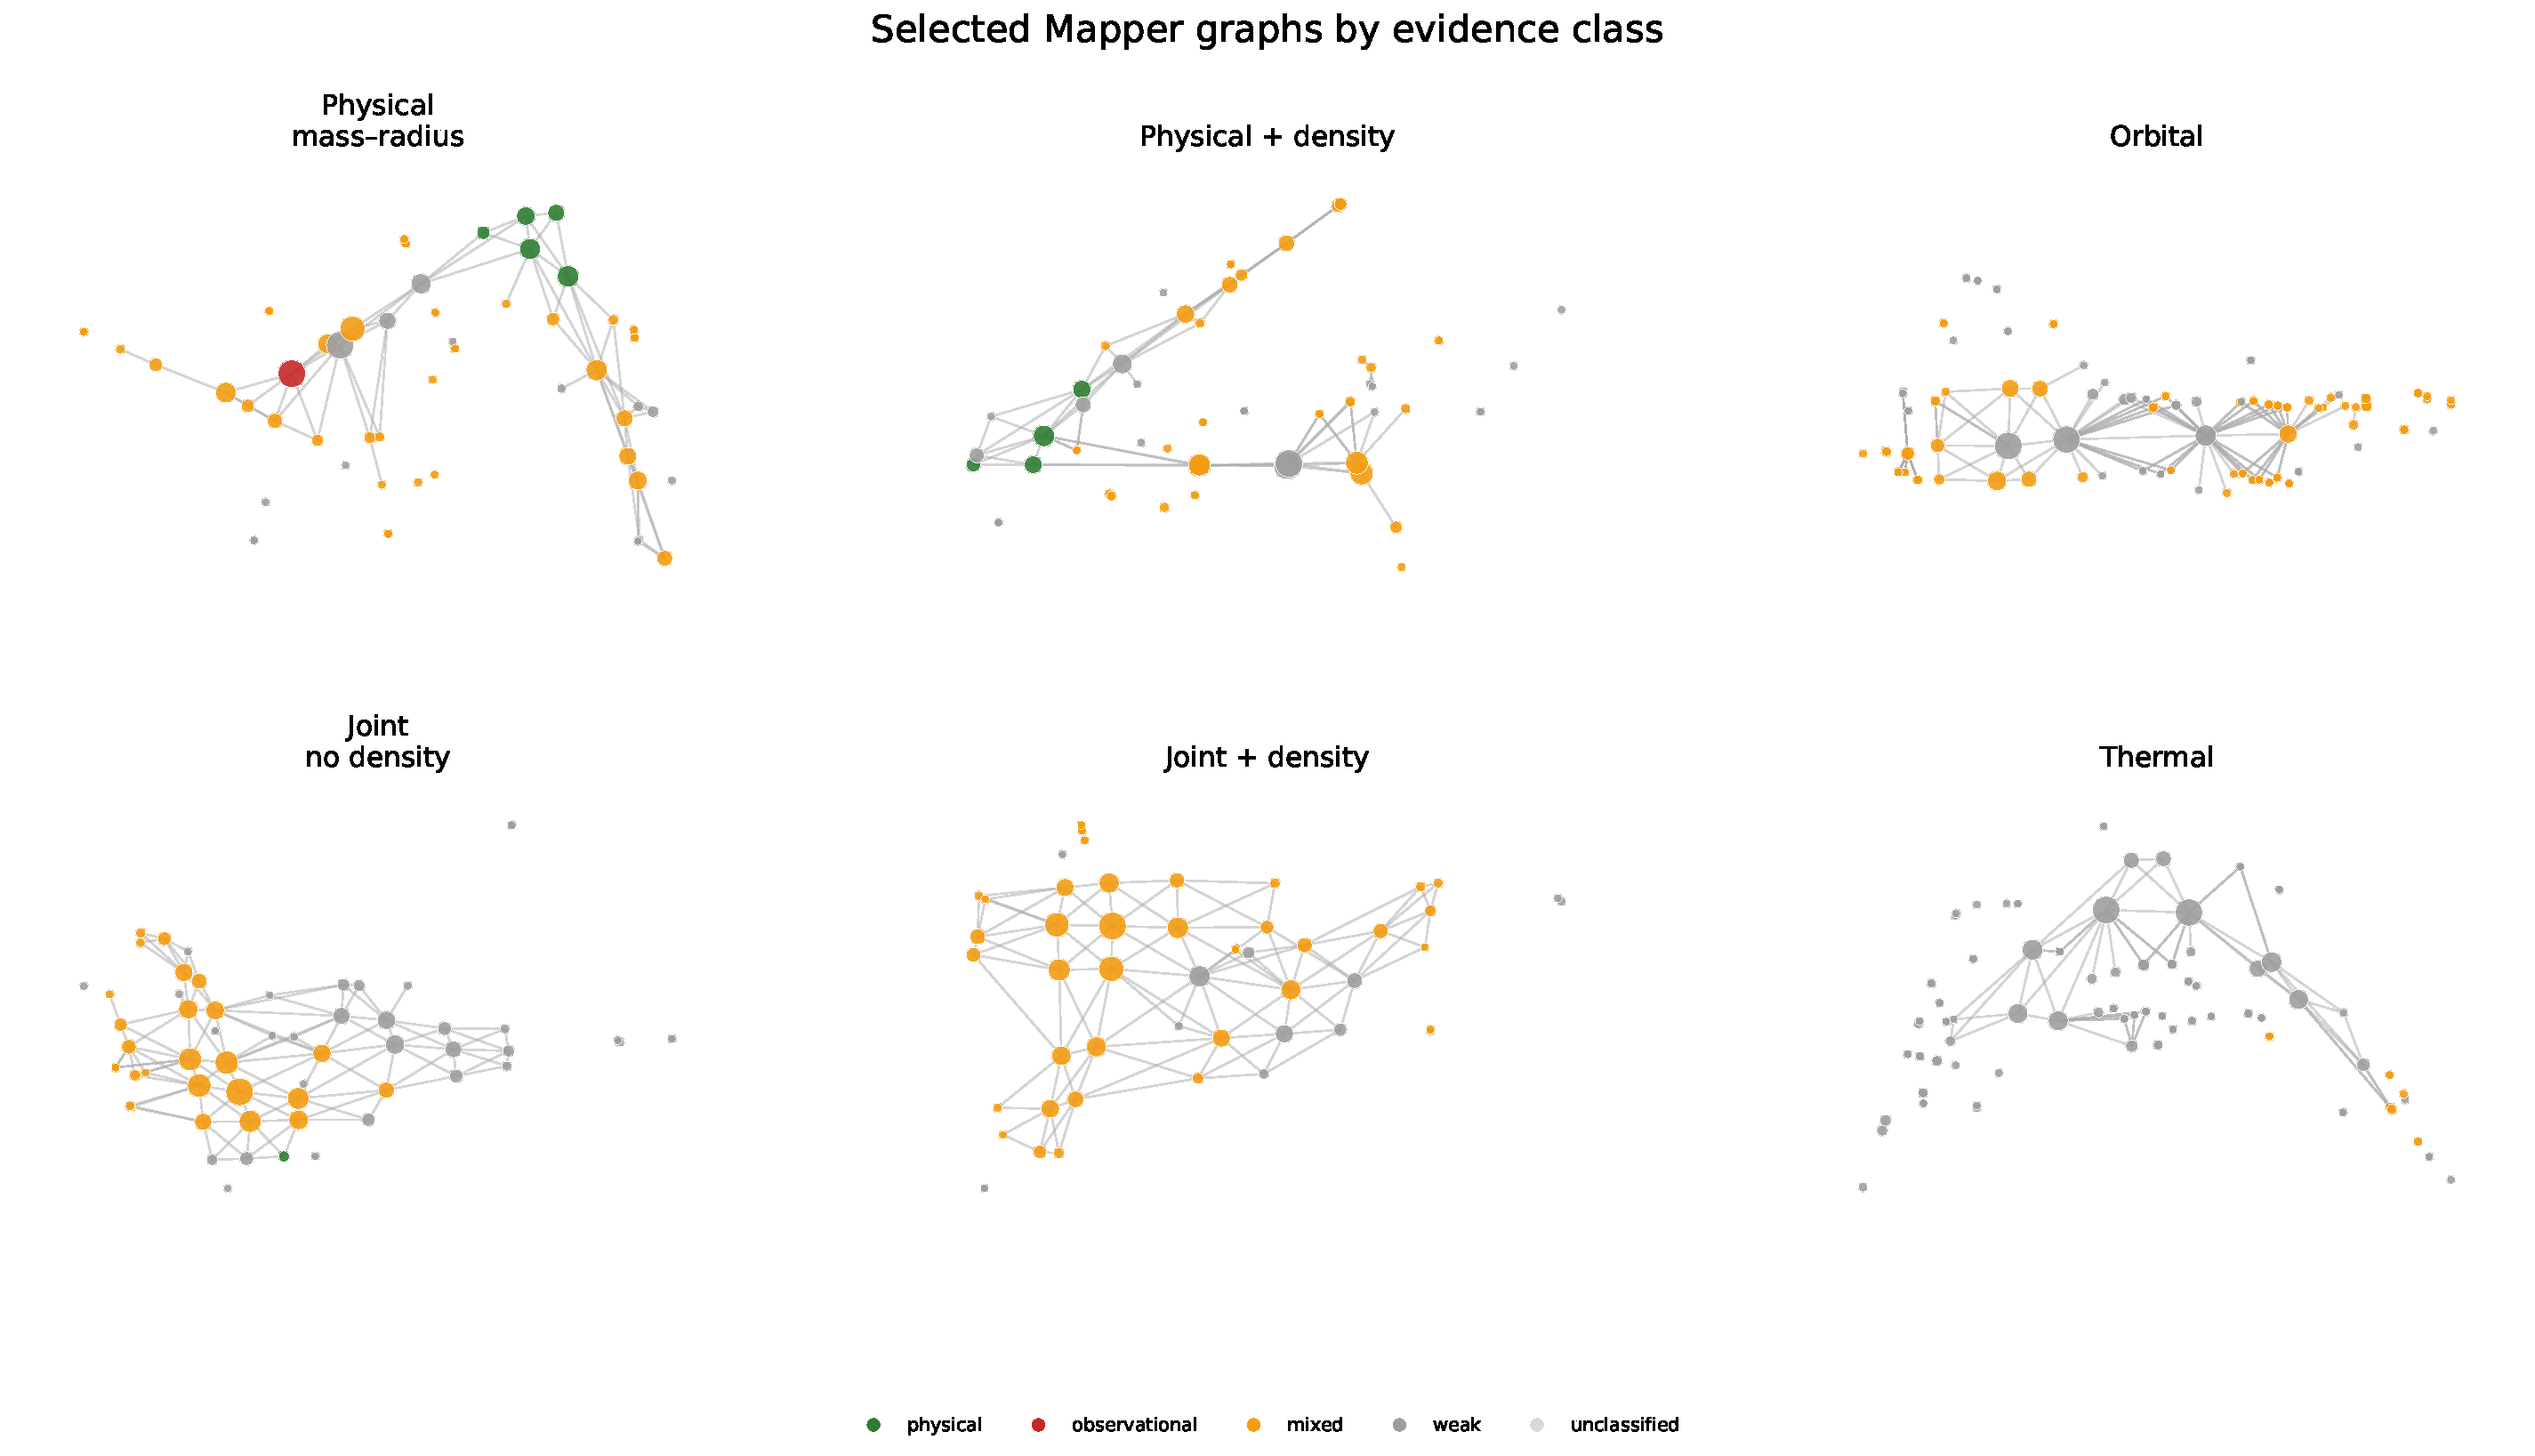
\includegraphics[width=0.95\linewidth]{figures/main_graphs_by_evidence_class.pdf}
\caption{Grafos Mapper seleccionados coloreados por categoría final de evidencia. Los colores distinguen regiones \texttt{physical}, \texttt{observational}, \texttt{mixed} y \texttt{weak}. La figura muestra que la estructura observada está dominada por regiones mixtas y débiles, mientras que las regiones físicas limpias son más escasas.}
\label{fig:main_graphs_by_evidence_class}
\end{figure}

La Figura~\ref{fig:main_graphs_by_evidence_class} es especialmente útil porque desplaza la lectura desde ``qué grafo se ve más complejo'' hacia ``qué tipo de evidencia sostiene cada región''. Un grafo puede tener muchos nodos y ciclos, pero si la mayoría de sus regiones son \texttt{mixed} o \texttt{weak}, la interpretación debe ser cautelosa. En cambio, las regiones \texttt{physical} son más valiosas como candidatas para inspección posterior porque combinan coherencia física u orbital con menor riesgo observacional y de imputación.

\subsection*{El caso del grafo orbital}

El grafo orbital sigue siendo el candidato principal del proyecto porque combina alta complejidad topológica con baja imputación. Tiene 124 nodos, 196 aristas, \(\beta_1=96\) e imputación media nodal de 0.011. Sin embargo, la síntesis final muestra que su interpretación no puede ser puramente astrofísica. La auditoría de \texttt{discoverymethod} mostró que su estructura tiene asociación significativa con el método de descubrimiento; por tanto, muchas regiones orbitales deben leerse como \texttt{mixed}.

\begin{figure}[H]
\centering
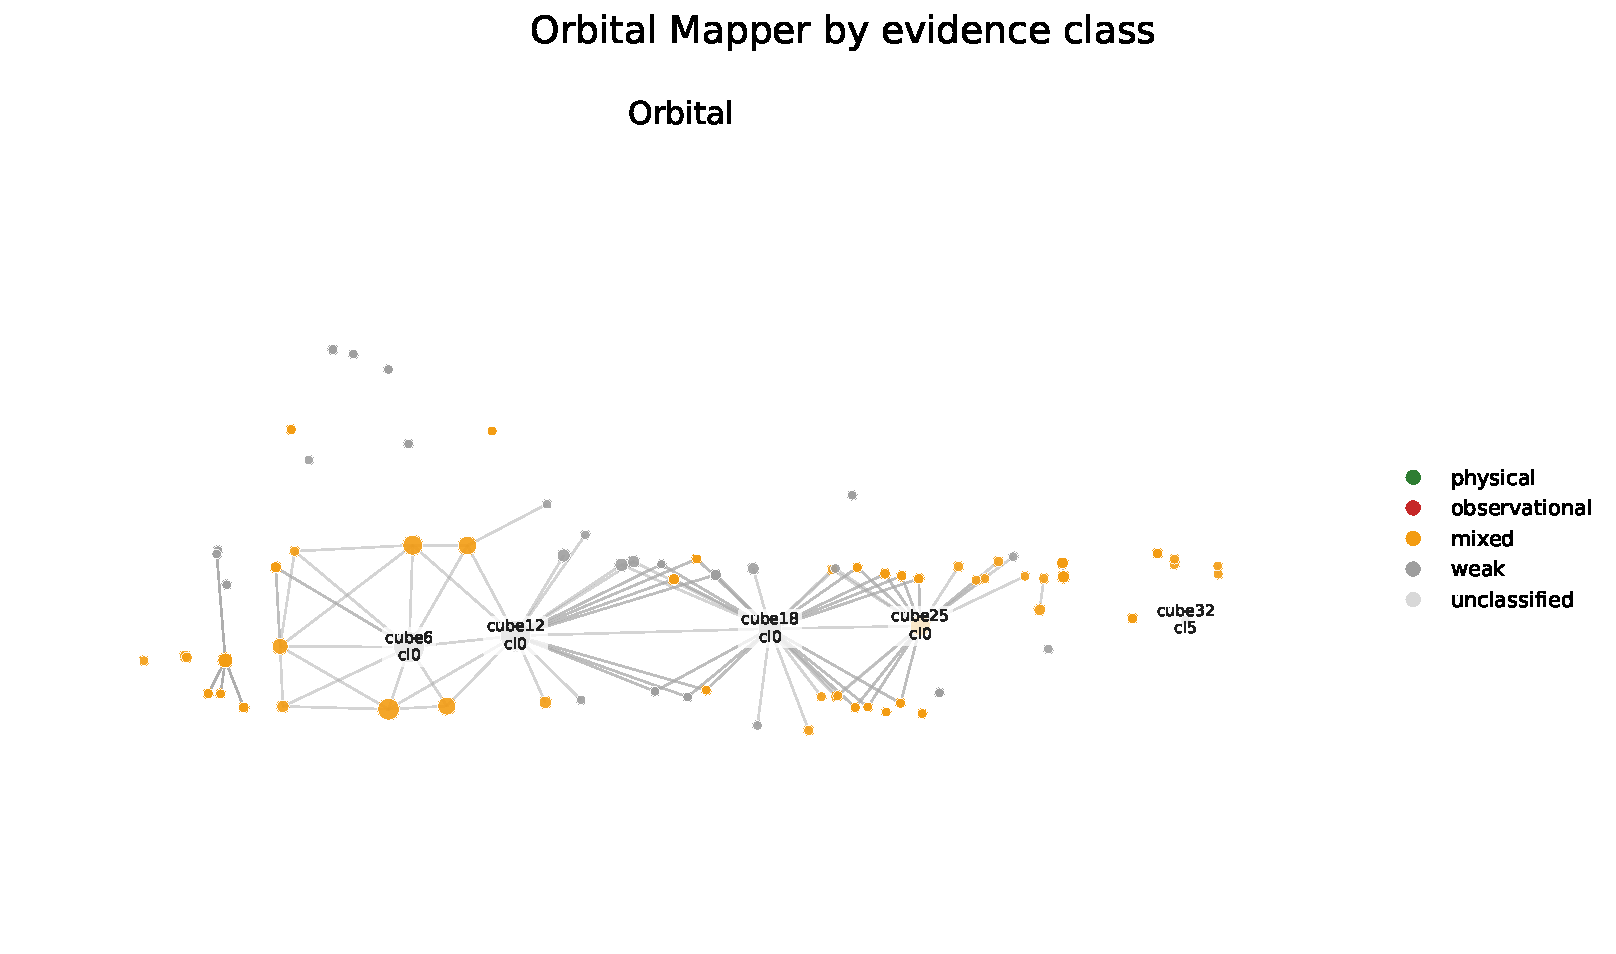
\includegraphics[width=0.78\linewidth]{figures/orbital_graph_evidence_class.pdf}
\caption{Grafo \texttt{orbital\_pca2\_cubes10\_overlap0p35} coloreado por categoría final de evidencia. Aunque el grafo orbital es el candidato más informativo por complejidad e imputación baja, muchas de sus regiones se interpretan como mixtas y no como señal orbital pura.}
\label{fig:orbital_graph_evidence_class}
\end{figure}

La Figura~\ref{fig:orbital_graph_evidence_class} muestra que el grafo orbital no debe resumirse simplemente como ``estructura física'' o ``sesgo''. Su valor está precisamente en la combinación: presenta estructura orbital informativa, pero esa estructura se intersecta con el proceso de descubrimiento. Esta lectura es consistente con el catálogo de exoplanetas: los planetas de periodo corto son más fáciles de detectar por tránsito, mientras que otros métodos favorecen regiones distintas del espacio físico y orbital.

Para distinguir mejor esa mezcla, se comparan dos visualizaciones adicionales del mismo grafo orbital: una por método de descubrimiento y otra por imputación.

\begin{figure}[H]
\centering
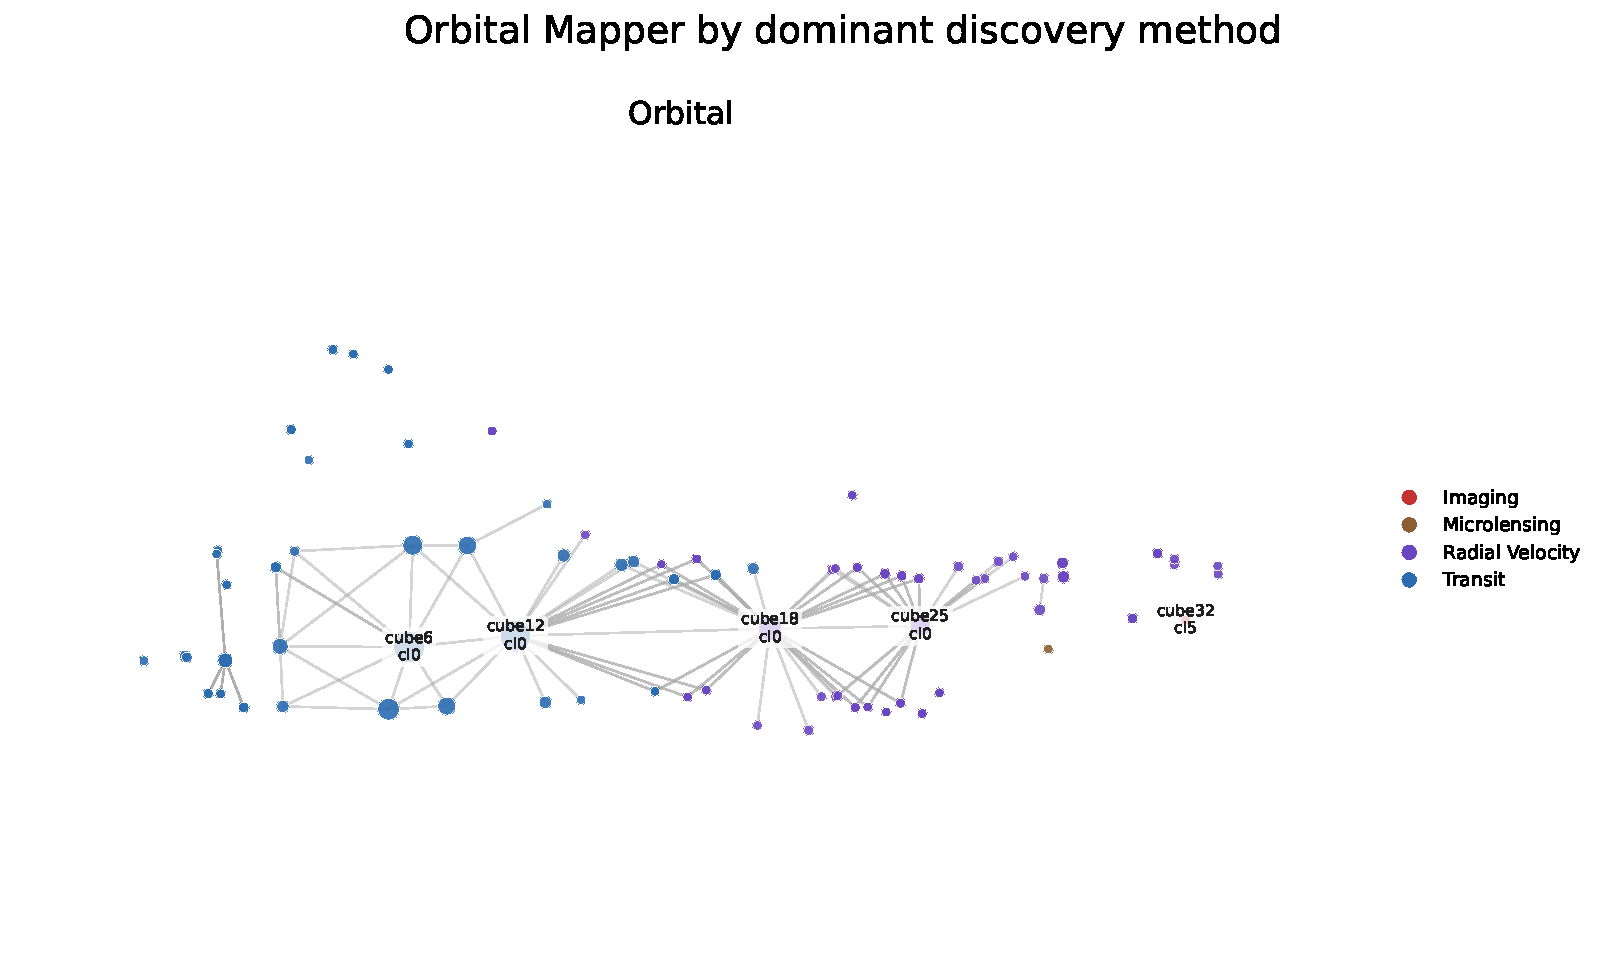
\includegraphics[width=0.78\linewidth]{figures/orbital_graph_discoverymethod.pdf}
\caption{Grafo orbital coloreado por método de descubrimiento dominante. La concentración de regiones por \texttt{discoverymethod} muestra que parte de la topología orbital está asociada con el proceso de detección.}
\label{fig:orbital_graph_discoverymethod}
\end{figure}

La Figura~\ref{fig:orbital_graph_discoverymethod} ayuda a interpretar por qué varias regiones orbitales terminan como \texttt{mixed}. Si ciertas zonas del grafo están dominadas por \texttt{Transit}, \texttt{Radial Velocity} o \texttt{Imaging}, entonces la estructura observada puede reflejar tanto arquitectura orbital como selección observacional. Esto no invalida el grafo orbital, pero sí impide interpretarlo como una señal orbital pura.

\begin{figure}[H]
\centering
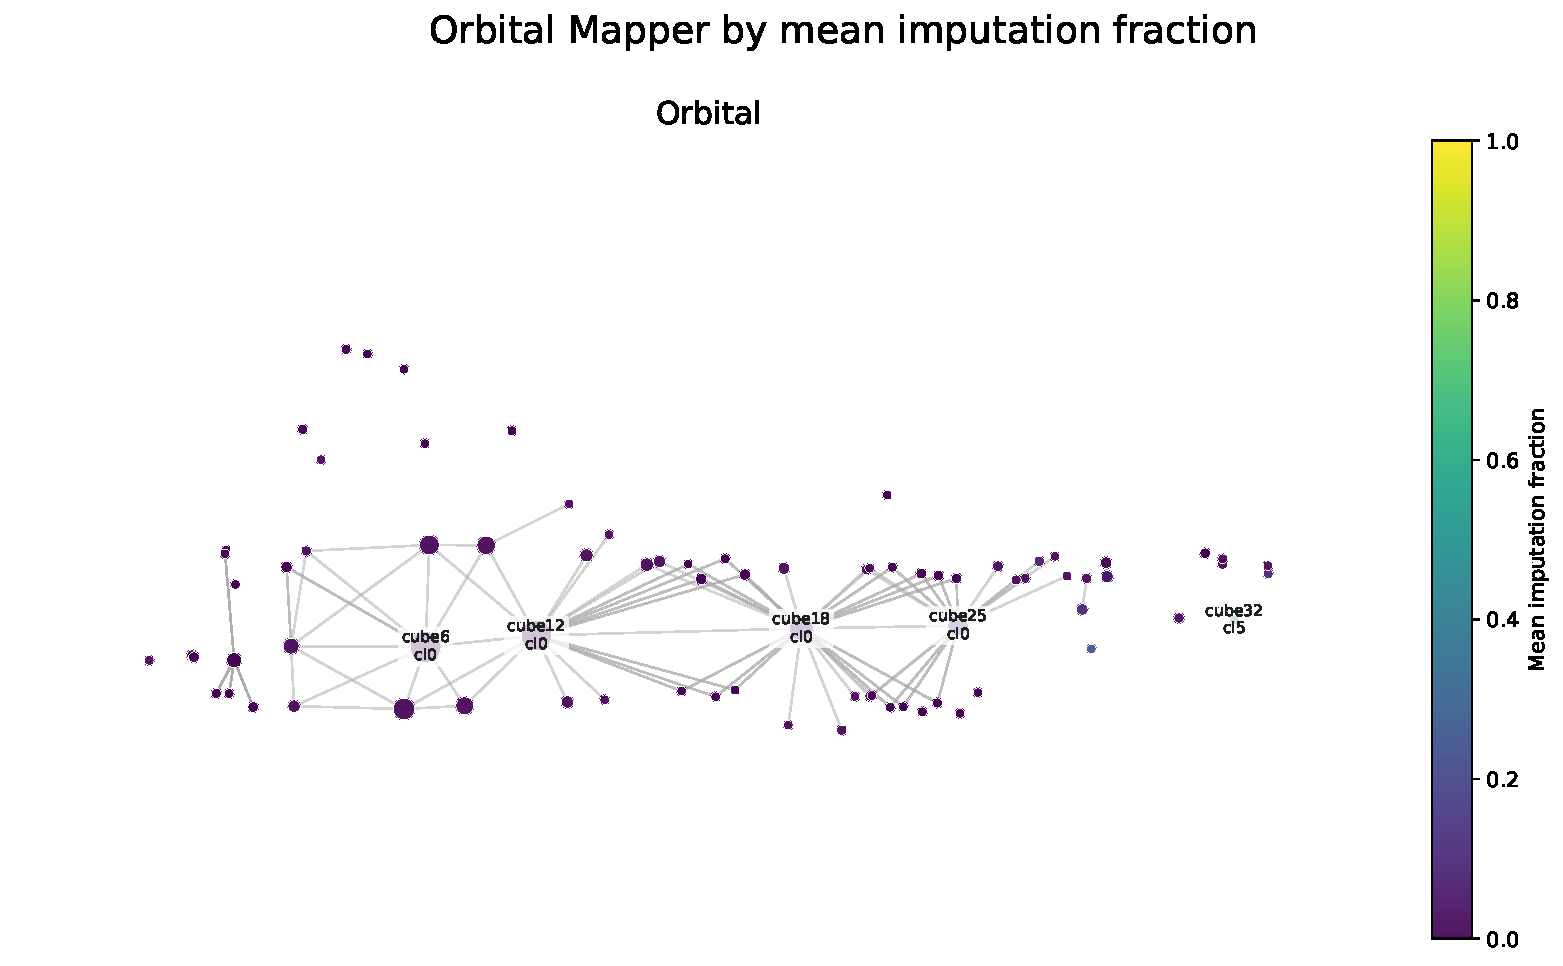
\includegraphics[width=0.78\linewidth]{figures/orbital_graph_imputation.pdf}
\caption{Grafo orbital coloreado por fracción de imputación. La baja imputación general del espacio orbital refuerza su valor como candidato de inspección, aunque la auditoría observacional obliga a una lectura mixta.}
\label{fig:orbital_graph_imputation}
\end{figure}

La Figura~\ref{fig:orbital_graph_imputation} muestra el otro lado de la interpretación. A diferencia del espacio térmico, el grafo orbital no está fuertemente sostenido por imputación. Por eso sigue siendo el resultado más informativo del proyecto. La tensión principal no es imputación, sino sesgo observacional: el grafo orbital es confiable en términos de datos, pero no independiente del proceso de descubrimiento.

\subsection*{Lectura de regiones \texttt{physical}}

Las regiones \texttt{physical} son las más defendibles para inspección científica posterior. En general, una región entra en esta categoría cuando muestra coherencia física u orbital, baja imputación y baja señal de enriquecimiento observacional. Estas regiones pueden corresponder a nodos con pureza de clase física relativamente alta, gradientes masa-radio coherentes o estructura orbital interpretable sin dominancia fuerte de un método de descubrimiento.

El número de regiones \texttt{physical} es bajo: 10 nodos. Esta escasez es importante. No significa que el catálogo no contenga señal astrofísica, sino que la evidencia limpia, bajo los criterios usados aquí, aparece en un subconjunto pequeño de regiones. En términos metodológicos, estas regiones son las mejores candidatas para inspección detallada, visualización individual y comparación con literatura astrofísica.

\subsection*{Lectura de regiones \texttt{observational}}

Las regiones \texttt{observational} aparecen cuando la evidencia está dominada por el proceso de descubrimiento. Esto puede ocurrir cuando una región tiene alta pureza por \texttt{discoverymethod}, baja entropía, enriquecimiento significativo bajo permutación, dominancia de una facilidad de descubrimiento o concentración temporal estrecha.

En los resultados finales, solo 1 nodo fue clasificado como \texttt{observational}, pero 4 componentes quedaron en esta categoría. Esto sugiere que las estructuras puramente observacionales son menos frecuentes que las mixtas, pero existen. Estas regiones no deben descartarse: también son científicamente informativas porque muestran cómo el catálogo está estructurado por la historia de observación. Sin embargo, no deben presentarse como evidencia física directa.

\subsection*{Lectura de regiones \texttt{mixed}}

La categoría \texttt{mixed} es la más importante para la interpretación global del proyecto. Una región \texttt{mixed} tiene algún patrón físico, orbital o térmico, pero también muestra señal observacional relevante. Esta categoría captura el comportamiento esperado en datos reales de exoplanetas: el catálogo no es una muestra uniforme de la población planetaria, sino el resultado de múltiples métodos, misiones, instrumentos y criterios de detección.

La abundancia de regiones \texttt{mixed} no significa que el análisis falló. Al contrario, muestra que Mapper está capturando estructuras que existen en el catálogo, pero que esas estructuras no pueden atribuirse de forma exclusiva a física planetaria. En particular, el grafo orbital cae en esta lectura: sigue siendo informativo por su complejidad y baja imputación, pero la asociación con \texttt{discoverymethod} obliga a interpretar muchas de sus regiones como mezcla de señal orbital y sesgo observacional.

\subsection*{Lectura de regiones \texttt{weak}}

Las regiones \texttt{weak} son aquellas donde la evidencia disponible no permite una interpretación fuerte. Esto puede deberse a alta imputación, tamaño pequeño del nodo o componente, evidencia física insuficiente, conflicto entre métricas o dependencia de variables menos confiables. Una región \texttt{weak} no significa que no exista estructura; significa que esa estructura no tiene soporte suficiente para sostener una conclusión astrofísica clara.

El número de nodos \texttt{weak} es alto: 245. Esto refuerza una de las lecciones metodológicas del proyecto. Mapper puede producir muchas regiones, pero no todas son igualmente interpretables. La síntesis final funciona precisamente como un filtro: evita que cada nodo del grafo sea tratado como una población significativa y prioriza únicamente aquellas regiones con mejor soporte.

\subsection*{Conclusión de la síntesis}

La síntesis final muestra que Mapper es útil para priorizar regiones de inspección, pero no para declarar una taxonomía final de exoplanetas. El predominio de regiones \texttt{mixed} y \texttt{weak} indica que la estructura observada está atravesada por sesgo observacional, imputación y decisiones metodológicas. Aun así, la presencia de regiones \texttt{physical} demuestra que sí existen candidatos con evidencia más limpia para análisis posterior.

El resultado principal de esta sección no es que Mapper descubra clases planetarias definitivas, sino que permite construir un mapa de evidencia. Bajo esta lectura, las regiones no se interpretan por su apariencia visual solamente, sino por la combinación de métricas que las sostienen. Esta es la contribución metodológica central del proyecto: separar estructura observada de interpretación astrofísica fuerte, y distinguir entre regiones físicas, observacionales, mixtas y débiles.